\documentclass[10pt,a4paper,twocolumn]{scrartcl}
\usepackage[utf8]{inputenc}
\usepackage[english]{babel}
\usepackage[T1]{fontenc}
\usepackage{amsmath}
\usepackage{amsfonts}
\usepackage{amssymb}
\usepackage{graphicx}
\usepackage{setspace}
\usepackage[left=2cm,right=2cm,top=2cm,bottom=2cm]{geometry}

\usepackage{booktabs}

\usepackage{hyperref}

\usepackage{natbib}
\bibliographystyle{alpha}
%\bibliographystyle{spr-chicago}
%\bibpunct[:\,]{(}{)}{;}{}{}{,}

\title{Reception of LGBT in Newspapers}
\author{Magdalena Bönisch \and Till Haubenreißer \and Maximilian Möller}
\publishers{\emph{Universität Leipzig, Introduction to Digital Humanities (Dr. Köntges)}}

\begin{document}
\onehalfspacing

\maketitle

{\footnotesize
\paragraph*{Abstract} Here are 150 to 200 words which constitute our abstract.
}


\section{Introduction}
This is our pretty Introduction.

\section{Workflow \& Implementation}
In the following, the general workflow for analyzing the LGBT reception within newspapers is described. After that, the concrete decisions concerning the implementation are addressed.

\subsection*{Workflow} The overall workflow is shown in Fig.~\ref{fig:workflow}. The upper part reflects the first step of collecting newspaper articles and creating a database. For each term from a predefined list of query terms an HTTP response to the API of an online newspaper archive is sent. In this work, the Article Search API of the New York Times\footnote{\url{https://developer.nytimes.com/}} is used as it provides access to articles published since its foundation in 1851 and thus enables an extensive time-dependent analysis. Furthermore, the returned JSON documents contain not only a URL to the actual article but also text snippets and lead paragraphs such that an analysis can be based on these text fields. Hence, no further call for the complete article is necessary. Besides meta-data like the number of hits, the API returns a JSON object consisting of the attribute-value pairs of the articles. Since the access to the NYT API is limited per second and per day, the responses are parsed and stored into a MySQL\footnote{\url{https://www.mysql.com/}} database. A relational database allows a quick access of the data along with SQL as a powerful query language for data selection and summarization. By using the database, subsequent analysis could be based on the whole corpus with no dependency from the API. Furthermore, the proposed workflow is more flexible with respect to adding data from an additional newspaper archive since its response has only to be mapped to schema of the database and, especially, the analysis module (lower part of the workflow in Fig.~\ref{fig:workflow}) remains unaffected.

\begin{figure}
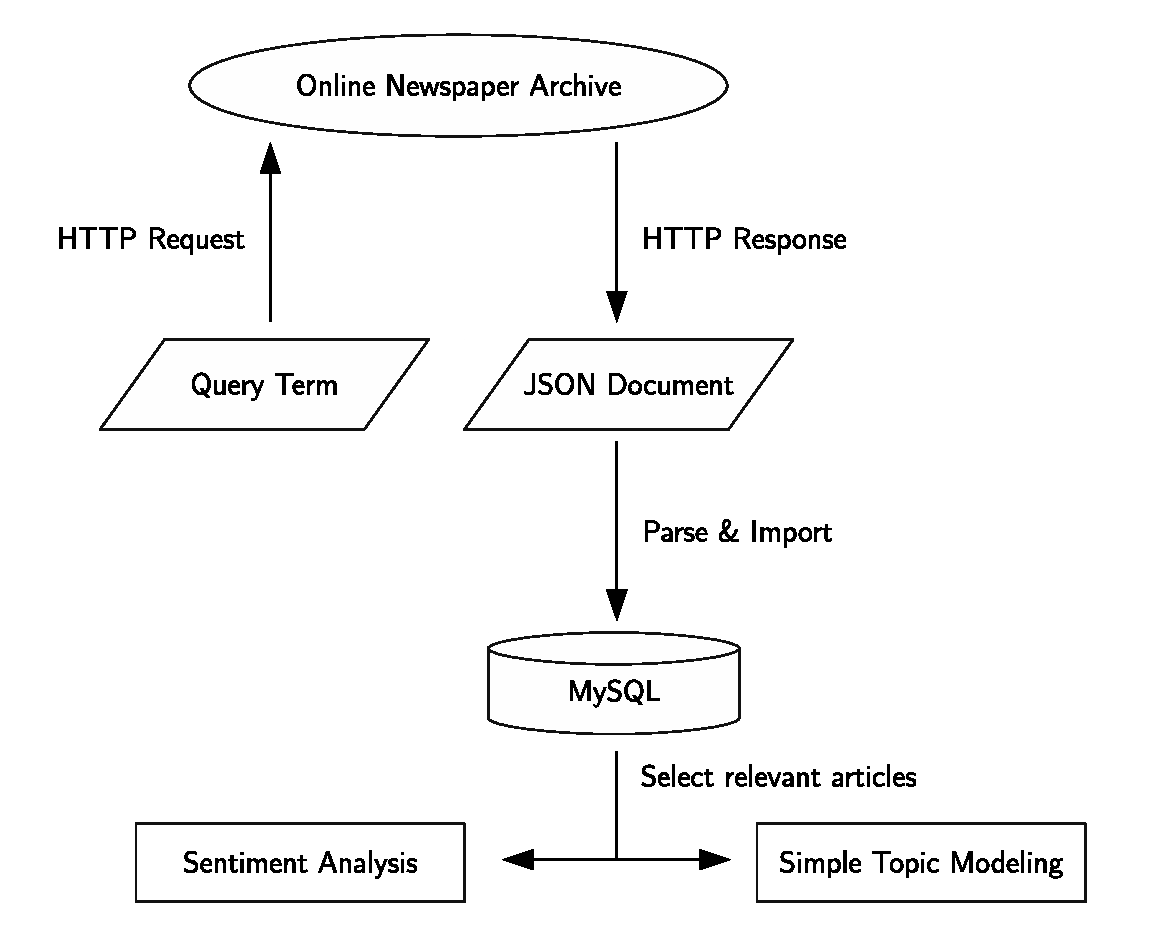
\includegraphics[width=\columnwidth]{figures/workflow_eps}
\caption{Workflow} \label{fig:workflow}
\end{figure}

The analyses are based on two dimensions: query term and time. Thus, the input of the sentiment analysis and the simplified topic modeling approach is a set of lead paragraphs containing the query term and contained in articles published at a certain time. For instance, such an input can be all paragraphs from the database which contain the word \textit{homosexual} and were published in the 1990s.

The sentiment analysis assigned each sentence a vector of sentiment probabilities. We considered five sentiments: \textit{very negative}, \textit{negative}, \textit{neutral}, \textit{positive}, and \textit{very positive}. For example, the vector \begin{center}
$v_s = \langle 0.2, 0.5, 0.1, 0.1, 0.1\rangle$
\end{center} describes the case that a sentence $s$ has a probability of $20\%$ for having a very negative sentiment, $50\%$ for having a negative sentiment, and $10\%$ for having a neutral, positive, and very positive sentiment, respectively. For the topic modeling, the joint occurrence of a target term together with another word (cooccurrence) is analyzed. Target terms are LGBT-related words, like the query terms.\footnote{The query terms are used for building an LGBT-corpus. But within this corpus it possible to search for other terms than query terms as well. For instance, \textit{lesbian} is a query term as well as a target term. \textit{gay} is only a target term.} Each cooccurrence is assigned its frequency and whether its occurrence is significant. For instance, the cooccurrence \begin{center}
$c_\text{2010s} = \langle \text{bisexual}, \text{rights}, 31, \text{true}\rangle$
\end{center} means that within the lead paragraphs from 2010 to 2019, \textit{bisexual} and \textit{rights} occurred 31-times in the same paragraph and that this occurrence is significant. By clustering significant cooccurrences, the topics were manually created in order to yield high-quality topics.

\subsection*{Implementation} The whole workflow is implemented in Java as a Maven\footnote{\url{https://maven.apache.org/}} project. The project is managed on GitHub.\footnote{\url{https://github.com/macksimiljan/lgbt-news}} It consists of one module for collecting and one for analyzing the data. The database is accessed by using the Java Database Connectivity (JDBC) API\footnote{\url{http://www.oracle.com/technetwork/java/javase/jdbc/index.html}}.

\paragraph*{Collecting Module} The used query terms are \textit{bisexual}, \textit{gay community}, \textit{homosexual}, \textit{lesbian}, \textit{transgender}, and \textit{transsexual}. However, the term \textit{gay} was not considered as a query term because it appeared too often in non-LGBT-related contexts like as a given name or surname. In order to obey the time limit of the NYT API, only one request per second was sent. Almost all requests ($95.4\%$) were successful. They returned a non-empty JSON object which could be inserted into the database. Failures of requests were due to denied accessed to the archive (HTTP 403) or gateway time-outs (HTTP 504). Because such failures were very rare, failed requests were not sent for a second time. All in all, the built corpus consists of $44,485$ articles whereby $93,7\%$ of them contain a non-empty lead paragraph on which the analyses are based.

The database models the mapping of query terms and keywords to articles. Keywords represent interesting additional information to the articles like associated persons, organizations, or geographical information. Approximately, $75\%$ of all articles have at least one keyword. Moreover, an article has a URL which leads to its HTML representation in two-thirds of the cases; otherwise the article is only accessible as a PDF document.\footnote{Older articles are archived as PDF not as HTML.} Further attributes are the publication date, the actual text type (for instance, article, interview, or biography) and headline, abstract, lead paragraph, and snippet. Since the headline is very short, the abstract is missing for $62\%$ of the articles, and the snippet is mostly the same as the lead paragraph, the analysis is based on the lead paragraph.

\paragraph*{Analysis Module} Essentially, the analysis module of the Maven project comprises the sentiment and the topic model package. They both rely on the sentence extraction task. For a certain search word and a certain publication date, this task selects windows of sentences from the paragraphs in the database. Given a window size of 2, for instance, additionally to the sentence containing the search word the two directly preceding as well the two directly succeeding sentences are extracted.\footnote{For the given corpus, a window size greater than 4 will have no difference to a smaller size since the paragraphs consists only of a few sentences. For instance, not more than 40\% of the paragraphs consists of two or more sentences.} For the sentiment analysis, we chose a window size of 0, i.e. only the containing sentence, and for the topic modeling a size of 1.  Both of the analyses depend on the natural language processing library Stanford CoreNLP\footnote{\url{http://stanfordnlp.github.io/CoreNLP/}}. This library contains annotators for tokenization, sentence splitting, part-of-speech tagging, and sentiment analysis. Since the sentiment annotator is based on the sentence structure, it is expected that it returns better results than approaches which only count the occurrences of particular negatively or positively connotated words or phrases while ignoring their syntactic context \citep{Socher+al:2013}. However, determining the sentence sentiment is a very time consuming operation. Therefore, we chose the minimal window size.

The simplified topic modeling approach consists of three steps: preprocessing, cooccurrence counting, and the statistic evaluation. The preprocessing is executed for the corpus only once. For all paragraphs, the contained words and their number of occurrence is determined. Stop words and numbers are excluded from this word statistics. The stop-word list is based on \citep[p.533]{Manning+Schuetze:2003} whereas numbers are recognized by a regular expression. After creating the word statistics, it is possible to define the list of context words. A context word is a meaningful word which occurs in a cooccurrence with a target word. A target word is a LGBT-related term. A word is assumed to be meaningful if it is not a stopword or a number and has a minimal frequency of 3. The frequency condition enforces that words being typographical errors are excluded from the analysis. After preprocessing, the word statistics consists of approximately $66\cdot 10^3$ word types and $1.2 \cdot 10^6$ word tokens.\footnote{Since we followed a simple approach, we did not run a lemmatizer. For comparison, the Oxford Dictionary counts about $200 \cdot 10^3$ (lemmatized) word types (inclusive stop words) in the English language \citep{Oxford}.}  $43.4\%$ of all words occur only once or twice. Thus, there are approximately $29\cdot 10^3$ context words.

In the next step, all cooccurences of a target word $w_\text{target}$ with one of the $n$ context words are counted in the paragraphs containing $w_\text{target}$ and published in a certain time span $t$. To yield the cooccurrences and their number, these paragraphs were tokenized and cleansed by removing all words from the sentences which are not context words and transforming it lower case. For instance, the sentences \begin{center}\textit{The president argues for gay rights. He is tolerant.}\end{center} is mapped to \begin{center}\textit{president argues gay rights tolerant}\end{center} This sequence of words is used to built a context vector $v_t(w_\text{target}) = \langle c_1, c_2, \ldots, c_n\rangle$ for each $w_\text{target}$ and $t$ such that $c_i$ represents the (absolute) frequency of the cooccurrence of $w_\text{target}$ with the context word at list position $i$. Because cooccurrence is not a reflexive relation between two words, $c_i = 0$ if the context word at position $i$ equals $w_\text{target}$. In the example, assume that the list of context words $L$ consists of six words: \begin{center}$L =  [\text{argues, gay, president, rights, tolerant, usa}]$\end{center} Depending on the chosen maximal distance $d_\text{max}$, the context vector $v_t(\text{gay})$ for the target word \textit{gay} is built. Let $d_\text{max}$ be 2, then there can no more than $d_\text{max} - 1 = 2 - 1 = 1$ word be between the target word and its cooccurrence partner. This yields the context vector \begin{center}$v_t^1(\text{gay}) = \langle 1, 0, 1, 1, 1, 0\rangle$\end{center} because every word except \textit{usa} occurs with \textit{gay} exactly once. For $d_\text{max} = 1$, only the direct neighbors of \textit{gay} are considered resulting in the context vector \begin{center}$v_t^2(\text{gay}) = \langle 1, 0, 0, 1, 0, 0\rangle$.\end{center} Studies suggest that the average sentence length in written prose is between 20 and 25 tokens, for instance \citep{Sichel:1974}. The maximal distance $d_\text{max}$ is not sentence-sensitive, i.e., it ignores sentence boundaries. Nevertheless, as the paragraphs are only a few sentences, there is a maximal distance $d'_\text{max}$ such that for all distances greater than $d'_\text{max}$ the number of cooccurrences is the same. Fig.~\ref{fig:distance} shows this for the count of cooccurrences with \textit{gay} in the 2010s. The number of all cooccurrences as well as the number of significant cooccurrences converge to 7650 and to 2300, respectively. These values are reached for a maximal distance greater than 56 (not shown in the figure). Tests with further target words lead to similar results. However, the smaller the maximal distance, the more semantically connected the words of the cooccurrence are expected to be. Choosing a great distance, the cooccurrences can connect words which probably are in different sentences. Since the sentence boundary is a semantic boundary as well (each sentence represents a logical statement on its own), a great maximal distance results in cooccurrences which might include words which should not be interpreted as being semantically connected. Thus, we run the program with a maximal distance of 6 and of 14 for all target words and times. For  $d_\text{max} = 6$ ($d_\text{max} = 14$), approximately $67\%$ ($85\%$) of all cooccurrences and $40\%$ ($67\%$) of all significant cooccurrences are detected. 


\begin{figure}
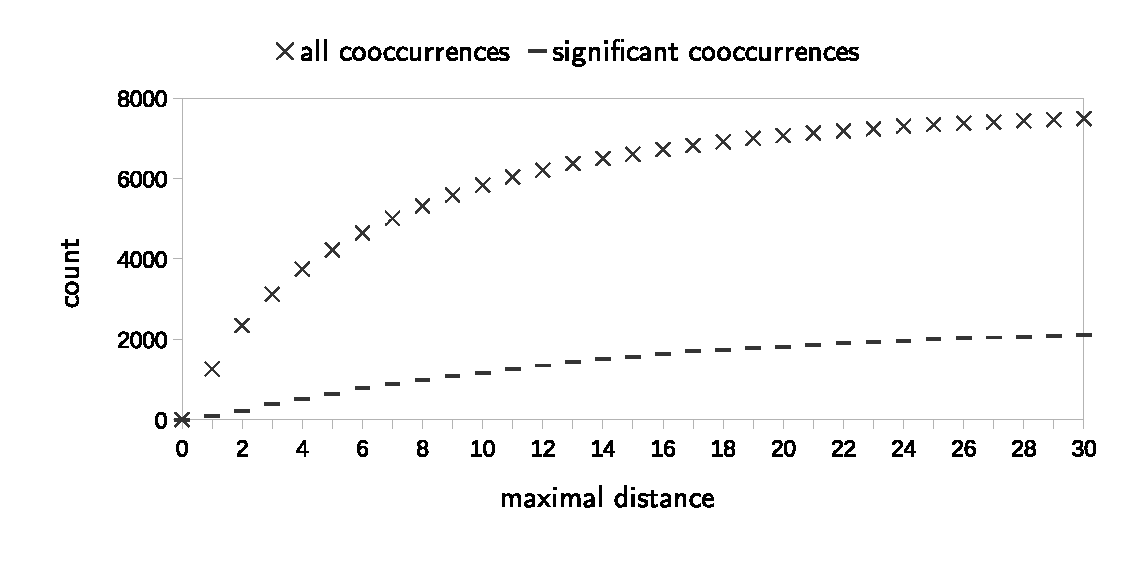
\includegraphics[width=\columnwidth]{figures/distance_eps}
\caption{Convergence of the number of cooccurrences.} \label{fig:distance}
\end{figure}

The last step is the calculation significant cooccurrences. According to \citep{Bordag2008, Manning+Schuetze:2003}, three significance measures were implemented: mutual information, log-likelihood, and t-score. For test data, the t-score yields the best results. Let $n$ be the number of context words, $n_\text{t}$ and $n_\text{c}$ the number of occurrences of the target word and of a context word, respectively. Furthermore, $n_{\text{t}\text{c}}$ is the count of the cooccurrence of $w_\text{target}$ and $w_\text{context}$. Then the t-score is defined according to Eq.~\ref{eq_tscore}.

\begin{equation}
\text{t}(w_\text{target}, w_\text{context}) = \frac{n_{\text{t}\text{c}} - \dfrac{n_\text{t} \cdot n_\text{c}}{n^2}}{\sqrt{n_{\text{t}\text{c}}}} \label{eq_tscore}
\end{equation}

 Consequently, a cooccurrence is defined as significant if it passes the t-test for $p = 0.005$. Additionally, all cooccurrences were selected occurring more often than on average in order to get further hints for topics. 

//TODO: keyword analysis

\section{Underlying Data}

\begin{table}
\centering
\caption{Size of the data basis.}
\begin{tabular}{lrr}
\toprule
term	 & \#articles & \#paragraphs\\
\midrule
bisexual &  $4,920$ & $2,973$\\
gay			& $-$ & $10,392$\\
gay community & $1,818$ & 377\\
homosexual  & $15,086$ & $5,263$\\
lesbian & $15,249$ & $5,086$\\
queer  & $-$ & 162\\
transgender  & $6,138$ & $2,973$\\
transsexual  & $1,229$ & 279\\
\bottomrule
\end{tabular}
\end{table}


\section{Results}

\subsection{Sentiment Analysis}
This is our spectacular sentimental analysis.

\subsection{Simple Topic Modeling}
This is our great topic modeling.

\section{Discussion}
This is our insightful discussion.

\subsection{Implementation Issues}
For comparing the reception of LGBT-related terms in different newspapers, it is necessary to integrate further newspaper articles into the database. Especially for The Guardian\footnote{\url{http://open-platform.theguardian.com/}}, this is no problem since the Guardian API returns less information than the NYT API, e.g. no publication date or lead paragraph. However, the most relevant information is the web URL to the article. Thus, in order to get the publication and textual information, the workflow has to be extended by a further request for receiving the HTML page of the full article as well as by a parser for extracting relevant information from this HTML document. When such an extension exists, it can be used to get the full article also from the NYT archive. The full article body would enable a more comprehensive topic modeling. Attention should be paid that the Guardian API provides only access to publication dating back to 1999.

A general problem with the newspaper archive APIs is that the access is limited. Assume that there are $150 \cdot 10^3$ articles for a certain query term; as it is the case for \textit{gay} in the NYT archive. Since the NYT API allows requesting only $10\cdot 10^3$ articles per day, collecting the whole result set takes 15 days. The same amount of articles is no bigger problem for the Guardian API where $250\cdot 10^3$ articles can be requested.\footnote{The Guardian allows $5\cdot 10^3$ calls per day and a maximum amount of 50 articles per call.} Additionally, only the first 1200 articles can be addressed within requests to the NYT API. Consequently, in order to get all articles, each call should not return more than that. In this approach, the articles of a query term were requested for a certain period of time.
 
// TODO: only cooccurrences of sentences? define max distance dynamically?
// TODO: count the distance from coWord to the targetWord

\subsection{Content Issues}

\subsection{Future Work}

\section{Conclusion}
This is our awesome conclusion.

{\footnotesize \bibliography{lit}}

\onecolumn

\newpage

\section*{Who did What?}

\renewcommand{\arraystretch}{1.5}
\begin{center}
\begin{tabular}{lccc}
\toprule
Task		& M. Bönisch & T. Haubenreißer & M. Möller\\
\midrule
general decisions & $\checkmark$ & $\checkmark$ & $\checkmark$\\
programming & & & $\checkmark$\\
basic data analysis  & & & $\checkmark$\\
diagram creation  & & $\checkmark$ &\\
background recherche & $\checkmark$ & $\checkmark$ & \\
evaluation of sentiment \\
topic evaluation\\
introduction text\\
workflow \& implementation text & & & $\checkmark$\\
underlying data text\\
results text\\
technical discussion text\\
content discussion text\\
future work text\\
conclusion text\\
typesetting  & & & $\checkmark$\\
\bottomrule
\end{tabular}
\end{center}
\renewcommand{\arraystretch}{1}

\end{document}